\documentclass[compress]{beamer}
%,hyperref={pdfpagelabels=false}

\usepackage[ngerman,english]{babel}
\usepackage[T1]{fontenc}
\usepackage[latin1]{inputenc}
\usepackage{amsmath}
\usepackage{amsthm}
\usepackage{amsfonts}
\usepackage{helvet}
\usepackage{url}
\usepackage{listings}
\usepackage{xcolor}
\usepackage{color}
\usepackage{xspace} % Abstand hinter Variablennamen
\usepackage{fix-cm}
%\usepackage[square, sort, numbers, authoryear]{natbib}

\usepackage{beamerthemeLEA2}

%\bibliographystyle{plainnat}

\newcommand{\N}       {\mathbb{N}}          % nat�rliche Zahlen
\newcommand{\Z}       {\mathbb{Z}}          % ganze Zahlen
\newcommand{\R}       {\mathbb{R}}          % reelle Zahlen
\newcommand{\Prob}    {\mathrm{P}}          % Wahrscheinlichkeit
\newcommand{\inter}   {\cap}                % Schnittmenge
\newcommand{\union}   {\cup}                % Vereinigung
\newcommand{\Oh}      {O}                   % O-Notation (Landau-Symbole)
\newcommand{\mycite}[1]{\textcolor{tumgreen}{[#1]}} 

\newenvironment{changemargin}[2]{% 
  \begin{list}{}{%
    \setlength{\topsep}{0pt}%
    \setlength{\leftmargin}{#1}%
    \setlength{\rightmargin}{#2}%
    \setlength{\listparindent}{\parindent}%
    \setlength{\itemindent}{\parindent}%
    \setlength{\parsep}{\parskip}%
  }%
  \item[]}{\end{list}}
  
\definecolor{light-gray}{gray}{0.95}
\definecolor{middle-gray}{gray}{0.5}
  
\lstset{basicstyle=\footnotesize\ttfamily,breaklines=true}
\lstset{columns=fullflexible}
\lstset{framextopmargin=20pt}
\lstset{backgroundcolor=\color{white}}
\lstset{escapeinside={<@}{@>}}

\title{A Flexible Tool for Shape Analysis}
\subtitle{IDP Presentation}
\author{\href{emanuel.laude@in.tum.de}{Emanuel Laude}\\ \href{laehner@in.tum.de}{Zorah L\"ahner} } 
%\date{\today}
\date{January 16, 2015}
\institute{Technische Universit�t M�nchen}

% Inhaltsverzeichnis zu Begin von jedem Abschnitt einblenden?
%\AtBeginSection[]{
%  \begin{frame}
%    \frametitle{Outline}
%    \tableofcontents[currentsection]
%  \end{frame}
%}

\begin{document}

\begin{frame}
  \titlepage
\end{frame}

% Inhaltsverzeichnis
\begin{frame}
  \frametitle{Outline}
  \tableofcontents
\end{frame}

\section{Demo Time}

\section{Class Overview}

\begin{frame}
  \frametitle{Class Diagram: View}
  \begin{figure}[h]
	\centering
	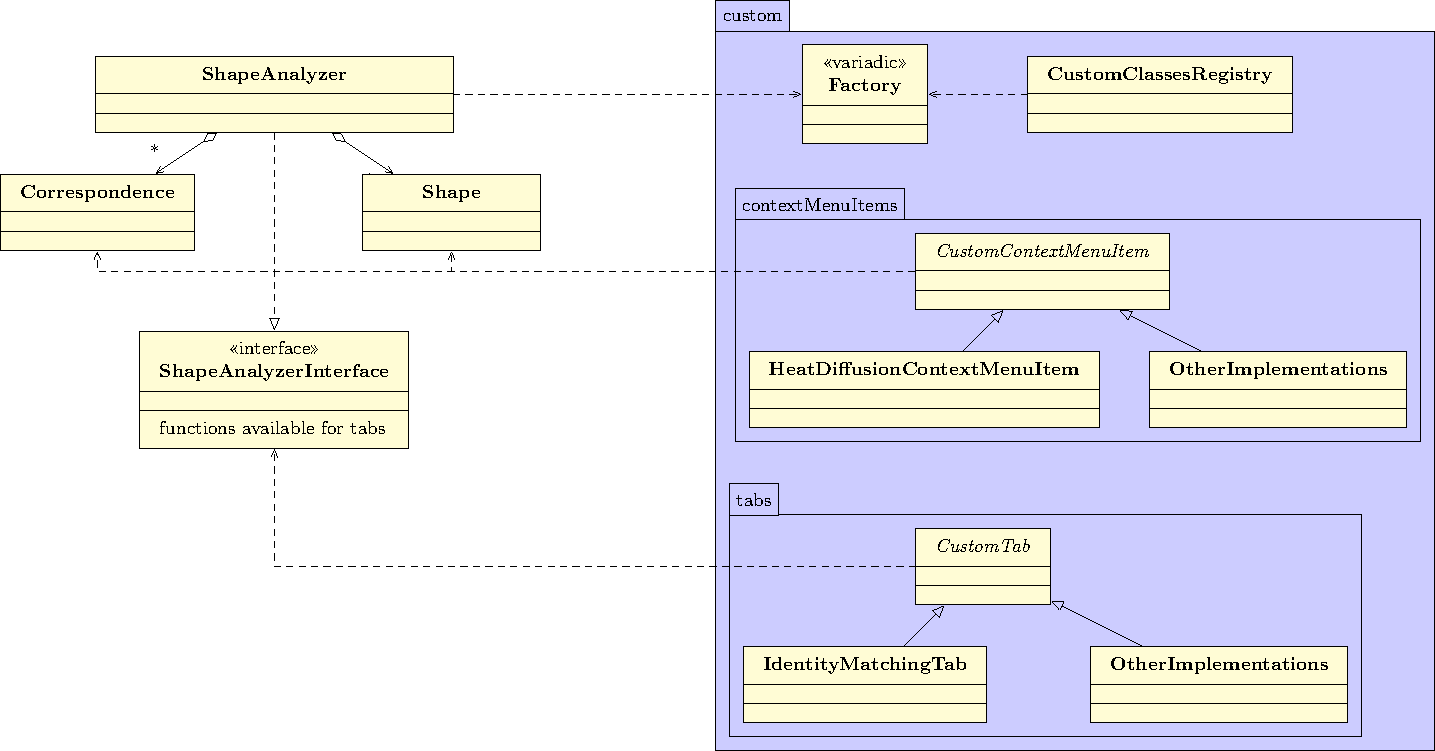
\includegraphics[width=\textwidth]{diagram.pdf}
\end{figure}
\end{frame}

\begin{frame}
  \frametitle{Class Diagram: Domain}
  \begin{figure}[h]
	\centering
	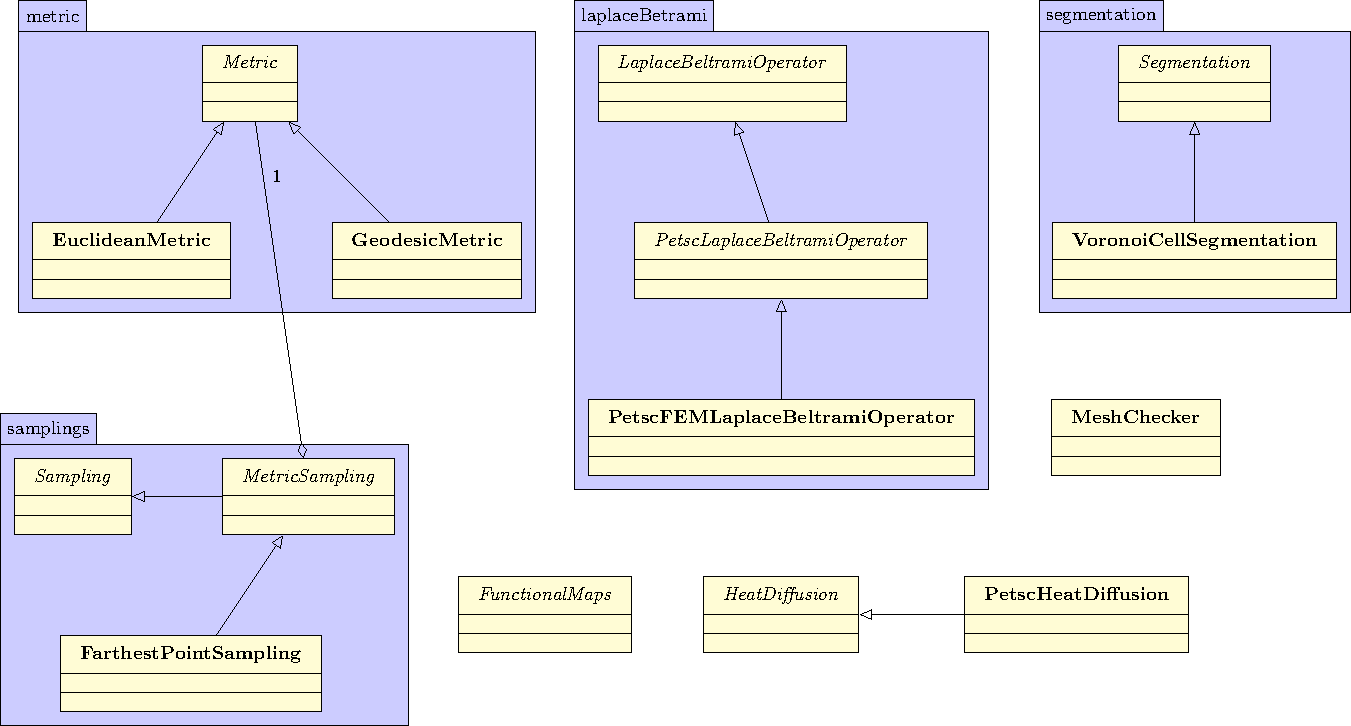
\includegraphics[width=\textwidth]{diagram2.pdf}
\end{figure}
\end{frame}

\section{Customs}

\begin{frame}[c]
  \frametitle{Customs}
  \begin{center}
  
  \huge CustomContextMenuItem 
  
  \vspace{1em}
  
  or 
  
  \vspace{1em}
  
  CustomTab?
  \end{center}
\end{frame}

\begin{frame}[fragile]
  \frametitle{Example: VoronoiCellsContextMenuItem}
  
\begin{lstlisting}[language=C++, numbers=none]
<@\textcolor{middle-gray}{template<class T = Metric>}@>
<@\textcolor{middle-gray}{class VoronoiCellsContextMenuItem : public CustomContextMenuItem \{}@>
<@\textcolor{middle-gray}{public:}@>
	<@\textcolor{middle-gray}{VoronoiCellsContextMenuItem<T>}@>
	<@\textcolor{middle-gray}{(shared\_ptr<Shape> shape, ShapeAnalyzerInterface* shapeAnalyzer)}@>
	 <@\textcolor{middle-gray}{: CustomContextMenuItem(shape, shapeAnalyzer) \{ \}}@>
    
    <@\textcolor{middle-gray}{virtual void onClick(vtkIdType pointId, vtkIdType faceId, QWidget* parent) \{}@>
        <@\textcolor{middle-gray}{(...)    \}}@>
<@\textcolor{middle-gray}{\};}@>
\end{lstlisting}
  
\end{frame}

\begin{frame}[fragile]
  \frametitle{Example: VoronoiCellsContextMenuItem}
  
\begin{lstlisting}[language=C++, numbers=none]
<@\textcolor{middle-gray}{template<class T = Metric>}@>
class VoronoiCellsContextMenuItem : public CustomContextMenuItem {
<@\textcolor{middle-gray}{public:}@>
	<@\textcolor{middle-gray}{VoronoiCellsContextMenuItem<T>}@>
	<@\textcolor{middle-gray}{(shared\_ptr<Shape> shape, ShapeAnalyzerInterface* shapeAnalyzer)}@>
	 <@\textcolor{middle-gray}{: CustomContextMenuItem(shape, shapeAnalyzer) \{ \}}@>
    
    <@\textcolor{middle-gray}{virtual void onClick(vtkIdType pointId, vtkIdType faceId, QWidget* parent) \{}@>
        <@\textcolor{middle-gray}{(...)    \}}@>
<@\textcolor{middle-gray}{\};}@>
\end{lstlisting}
  
\end{frame}

\begin{frame}[fragile]
  \frametitle{Example: VoronoiCellsContextMenuItem}
  
\begin{lstlisting}[language=C++, numbers=none]
template<class T = Metric>
<@\textcolor{middle-gray}{class VoronoiCellsContextMenuItem : public CustomContextMenuItem \{}@>
<@\textcolor{middle-gray}{public:}@>
	<@\textcolor{middle-gray}{VoronoiCellsContextMenuItem<T>}@>
	<@\textcolor{middle-gray}{(shared\_ptr<Shape> shape, ShapeAnalyzerInterface* shapeAnalyzer)}@>
	 <@\textcolor{middle-gray}{: CustomContextMenuItem(shape, shapeAnalyzer) \{ \}}@>
    
    <@\textcolor{middle-gray}{virtual void onClick(vtkIdType pointId, vtkIdType faceId, QWidget* parent) \{}@>
        <@\textcolor{middle-gray}{(...)    \}}@>
<@\textcolor{middle-gray}{\};}@>
\end{lstlisting}
  
\end{frame}

\begin{frame}[fragile]
  \frametitle{Example: VoronoiCellsContextMenuItem}
  
\begin{lstlisting}[language=C++, numbers=none]
<@\textcolor{middle-gray}{template<class T = Metric>}@>
<@\textcolor{middle-gray}{class VoronoiCellsContextMenuItem : public CustomContextMenuItem \{}@>
<@\textcolor{middle-gray}{public:}@>
	VoronoiCellsContextMenuItem<T>
	 (shared_ptr<Shape> shape, ShapeAnalyzerInterface* shapeAnalyzer)
	 	: CustomContextMenuItem(shape, shapeAnalyzer) { }
    
    <@\textcolor{middle-gray}{virtual void onClick(vtkIdType pointId, vtkIdType faceId, QWidget* parent) \{}@>
        <@\textcolor{middle-gray}{(...)    \}}@>
<@\textcolor{middle-gray}{\};}@>
\end{lstlisting}
  
\end{frame}

\begin{frame}[fragile]
  \frametitle{Example: VoronoiCellsContextMenuItem}
  
\begin{lstlisting}[language=C++, numbers=none]
<@\textcolor{middle-gray}{template<class T = Metric>}@>
<@\textcolor{middle-gray}{class VoronoiCellsContextMenuItem : public CustomContextMenuItem \{}@>
<@\textcolor{middle-gray}{public:}@>
	<@\textcolor{middle-gray}{VoronoiCellsContextMenuItem<T>}@>
	<@\textcolor{middle-gray}{(shared\_ptr<Shape> shape, ShapeAnalyzerInterface* shapeAnalyzer)}@>
	 <@\textcolor{middle-gray}{: CustomContextMenuItem(shape, shapeAnalyzer) \{ \}}@>
    
    virtual void onClick(vtkIdType pointId, vtkIdType faceId, QWidget* parent) {
        (...)    }
<@\textcolor{middle-gray}{\};}@>
\end{lstlisting}
  
\end{frame}

\begin{frame}[fragile]
  \frametitle{Example: VoronoiCellsContextMenuItem}
  
\begin{lstlisting}[language=C++, numbers=none]
virtual void onClick(...) {
        bool ok;
        vtkIdType source = QInputDialog::getInt(...);
        if (!ok) { return; }
        (...)
        if(ok) {
            try {
                auto m = make_shared<T>(shape_);
                auto fps = make_shared<FarthestPointSampling>(shape_, m, source, numberOfSegments);
                VoronoiCellSegmentation segmentation(shape_, m, fps);
                
                shape_->setColoring(segmentation.getSegments(), Shape::Coloring::Type::PointSegmentation);
            } catch(metric::MetricError& e) {
                QMessageBox::warning(parent, "Exception", e.what());
            }
        }
    }
\end{lstlisting}
  
\end{frame}

\section{Demo Time: Functional Maps}

\begin{frame}
  \frametitle{Example:}
  
\end{frame}

\end{document}
